\documentclass[11pt,letterpaper]{article}
\usepackage[margin=1in]{geometry}
\usepackage{amsmath,amssymb}
\usepackage{graphicx}
\usepackage{booktabs}
\usepackage[hidelinks]{hyperref}

\setlength{\parindent}{0pt}
\setlength{\parskip}{0.6em}
\setcounter{tocdepth}{1}

\newcommand{\tasksection}[2]{
    \clearpage
    \phantomsection
    \section*{#1: #2}
    \addcontentsline{toc}{section}{#1: #2}
}

\title{Project 2 Report\\[0.4em]
    \large CMPEN/EE 454}
\author{Mingcheng Liang, TianKuo Liao, Yuxin Liu\\}
\date{2026/10/28}

\begin{document}

\maketitle
Numerical results in this report are recorded in \texttt{README.md}. Displayed values are rounded where indicated. World coordinates are in millimeters and image coordinates are in pixels.
\tableofcontents

\subsection*{Team contributions}
\begin{center}
\begin{tabular}{ll}
\toprule
Team member & Tasks completed \\
\midrule
TianKuo Liao & Task 3.1 \\
Yuxin Liu & Task 3.5, Report \\
Mingcheng Liang & Tasks 3.2, 3.3, 3.4, 3.6, 3.7, Extra Task 1, Report \\
\bottomrule
\end{tabular}
\end{center}

\tasksection{Task 3.1}{Camera Parameters}
\label{sec:task3-1}

\subsection*{Intrinsic and extrinsic parameters}
The camera structures contain the intrinsic fields \texttt{foclen} ($f$), \texttt{prinpoint} ($(c_x,c_y)$), \texttt{aspectratio} ($a$), and \texttt{skew} ($s$). The extrinsic fields describe the camera center \texttt{position} ($\mathbf{C}$) and its orientation. The field \texttt{orientation} is a unit quaternion; our equations use its rotation-matrix representation, \texttt{Rmat} ($R$).

The function \texttt{task3\_1} constructs the intrinsic matrix as
\[
    K = \begin{bmatrix}
        fa & s & c_x\\
        0 & f & c_y\\
        0 & 0 & 1
    \end{bmatrix}.
\]
The parameters printed for the two cameras are:
\begin{center}
\begin{tabular}{lrr}
\toprule
Parameter & Camera 1 & Camera 2 \\
\midrule
$f$ (pixels) & 1560.6793 & 1527.9015 \\
$c_x$ (pixels) & 967.5391 & 969.8920 \\
$c_y$ (pixels) & 548.7386 & 549.8908 \\
$a$ & 1.0000 & 1.0000 \\
$s$ (pixels) & 0.0000 & 0.0000 \\
\bottomrule
\end{tabular}
\end{center}

\subsection*{Camera centers and the extrinsic matrix}
The \texttt{position} field gives the camera center in world coordinates:
\[
\begin{aligned}
    \mathbf{C}_1 &= (-4479.6412,\ 5524.6708,\ 1899.0398)^T\ \mathrm{mm},\\
    \mathbf{C}_2 &= (4416.8864,\ 5513.7913,\ 1788.9126)^T\ \mathrm{mm}.
\end{aligned}
\]
A world point is first translated relative to the camera center and then rotated into the camera frame:
\[
    \mathbf{X}_{\mathrm{cam}}=R(\mathbf{X}-\mathbf{C}) = \begin{bmatrix}
        R & -R \mathbf{C}
    \end{bmatrix}
      \begin{bmatrix}
        \mathbf{X} \\ 1
    \end{bmatrix}.
\]
Thus, \texttt{Pmat} is the $3\times4$ extrinsic matrix $[R\mid -R\mathbf{C}]$; the full pixel projection matrix is $K\,\texttt{Pmat}$.

For verification, \texttt{task3\_1} subtracts the reconstructed matrices from the stored \texttt{Kmat} and \texttt{Pmat}. Both intrinsic differences are exactly zero. The largest absolute extrinsic differences in the recorded run are approximately $9.095\times10^{-13}$ for camera 1 and $1.137\times10^{-13}$ for camera 2. These negligible residuals confirm the expected relationship between \texttt{position}, \texttt{Rmat}, and \texttt{Pmat}.

\tasksection{Task 3.2}{Projection of 3D Points}
\label{sec:task3-2}

\subsection*{Projection model and implementation}
We projected the 39 mocap points into both corrected images. For camera $j$, a world point $\widetilde{\mathbf{X}}=[X,Y,Z,1]^T$ is mapped to a homogeneous image vector
\[
    \mathbf{q}_j = K_j\,\texttt{Pmat}_j\,\widetilde{\mathbf{X}},
    \qquad
    (u_j,v_j) = \left(\frac{q_{j1}}{q_{j3}}, \frac{q_{j2}}{q_{j3}}\right).
\]

In the implementation, \texttt{mocap\_data.pts3D} is a $3\times39$ array. Appending a row of ones gives a $4\times39$ array, so all points can be projected at once with matrix multiplication and element-wise division. The returned arrays, \texttt{pts2d\_1} and \texttt{pts2d\_2}, each have size $2\times39$ and retain the original correspondence order. They are used for triangulation in Task 3.3 and evaluation in Task 3.7.

\subsection*{Visual verification}
Figure~\ref{fig:task32-projection} shows the red projected points on the two images.
\begin{figure}[!htbp]
    \centering
    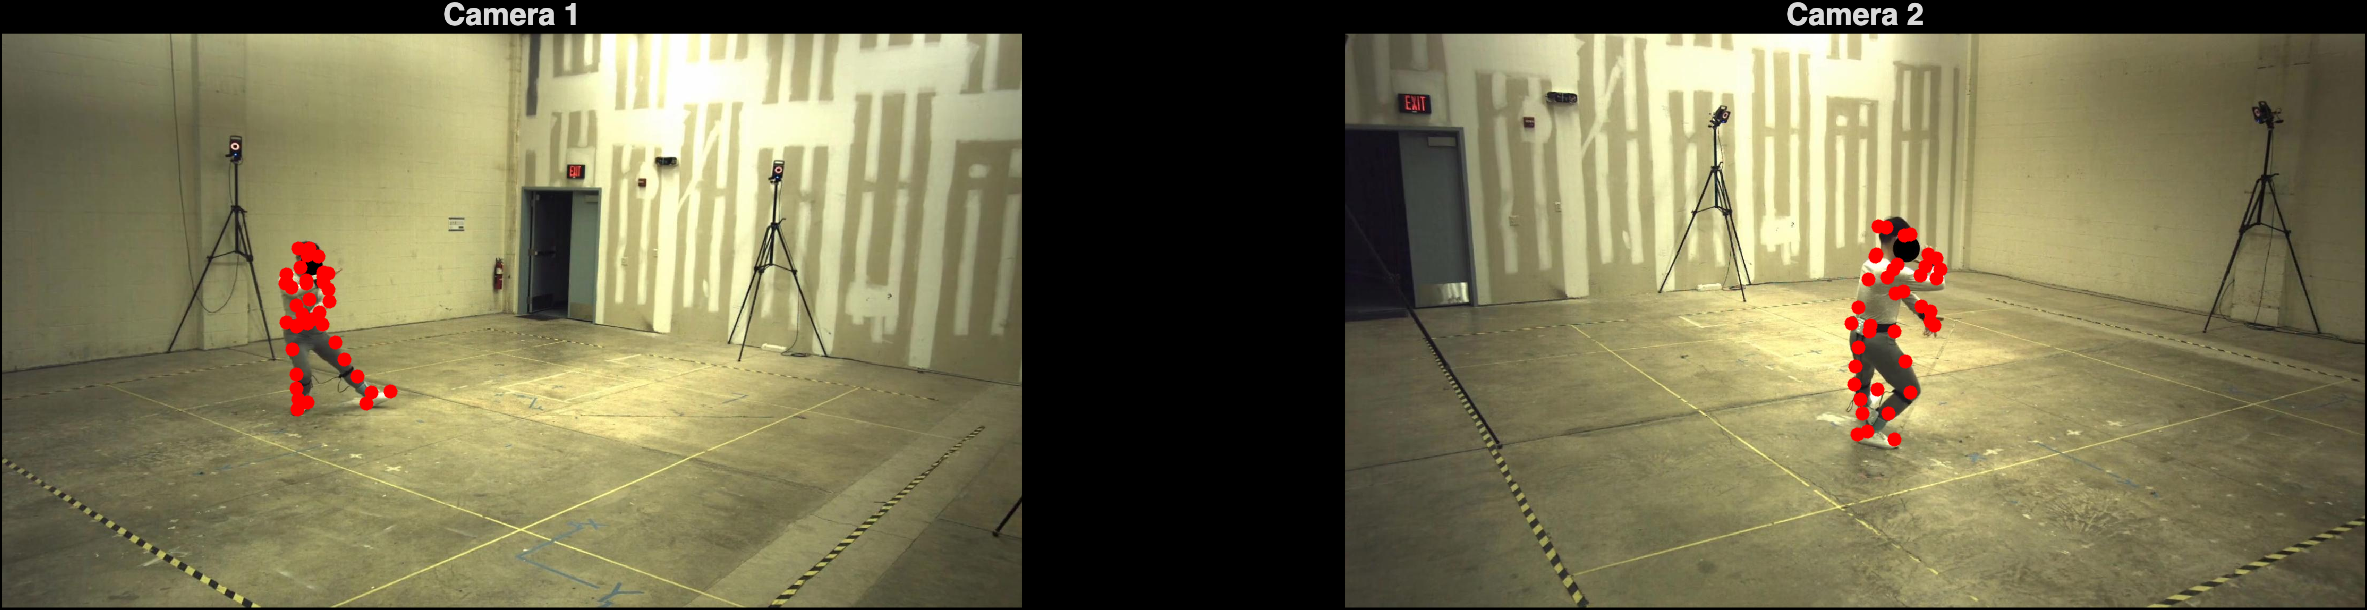
\includegraphics[width=\textwidth]{figures/task3-2-projection.png}
    \caption{The 39 mocap points projected by \texttt{task3\_2}. Left: camera 1. Right: camera 2.}
    \label{fig:task32-projection}
\end{figure}

\tasksection{Task 3.3}{3D Reconstruction by Triangulation}
\label{sec:task3-3}

\subsection*{Objective and projection model}
Task 3.2 produces two sets of corresponding pixel locations by projecting the 39 mocap points into the two camera views. In this task, each pair is used to reconstruct a 3D point, which is then compared with its original mocap position.

For camera $j\in\{1, 2\}$, use the full pixel projection matrix:
\[
    P_j = K_j \, \texttt{Pmat}_j \in \mathbb{R}^{3 \times 4}.
\]
Here, $K_j$ is the intrinsic matrix and $\texttt{Pmat}_j$ is the world-to-camera extrinsic matrix. A world point $\widetilde{\mathbf{X}}=[X,Y,Z,1]^T$ and its corresponding pixel $\widetilde{\mathbf{x}}_j=[u_j,v_j,1]^T$ satisfy:
\[
    \lambda_j \widetilde{\mathbf{x}}_j = P_j \widetilde{\mathbf{X}},
    \qquad j = 1, 2,
\]
where $\lambda_j$ is the projective scale. 

Ideally, the two back-projected rays intersect at the original 3D point. However, measurement noise or numerical errors may prevent an exact intersection. We therefore reconstruct the 3D point using linear triangulation based on the Direct Linear Transformation (DLT) method, with the homogeneous system solved using Singular Value Decomposition (SVD).

\subsection*{Linear triangulation and SVD implementation}

Write the rows of $P_j$ as $p_{j1}^T , p_{j2}^T , p_{j3}^T$. Eliminating $\lambda_j = p_{j3}^T \widetilde{\mathbf{X}}$ gives two linear constraints per camera:
\[
    (u_j p_{j3}^T - p_{j1}^T)\widetilde{\mathbf{X}}=0,
    \qquad
    (v_j p_{j3}^T - p_{j2}^T)\widetilde{\mathbf{X}}=0.
\]
Combining both views yields a $4\times4$ homogeneous system,
\[
    A\widetilde{\mathbf{X}}=0,
    \qquad
    A=\begin{bmatrix}
        u_1 p_{13}^T - p_{11}^T\\
        v_1 p_{13}^T - p_{12}^T\\
        u_2 p_{23}^T - p_{21}^T\\
        v_2 p_{23}^T - p_{22}^T
    \end{bmatrix}.
\]
In an ideal noise-free and non-degenerate case, $A$ has rank three and its null space determines the point up to scale. But with numerical error or noisy coordinates, we need to solve the constrained algebraic least-squares problem:
\[
    \widehat{\mathbf{h}} = \underset{\| \mathbf{h} \|_2 = 1}{\operatorname{argmin}}\| A \mathbf{h} \|_2^2.
\]
The constraint excludes the trivial solution. 

Let
$A = U \Sigma V^T$ with singular values $\sigma_1 \geq \sigma_2 \geq \sigma_3 \geq \sigma_4 \geq 0$. Since $A \mathbf{v}_k = \sigma_k \mathbf{u}_k$, the minimum is attained by
$\widehat{\mathbf{h}}=\mathbf{v}_4$, the last column of $V$.

The resulting homogeneous solution is converted to Euclidean 3D coordinates by:
\[
\widehat {\mathbf{X}} = 
\left[
\frac{h_1}{h_4},
\frac{h_2}{h_4},
\frac{h_3}{h_4}
\right]^T.
\]

This produces the reconstructed 3D point in the world coordinate.

\clearpage

\subsection*{Verification against the mocap points}
To verify reconstruction, we pass the two projected point arrays from Task 3.2 in their original correspondence order to the triangulation function. The output $\widehat{\mathbf{X}}_i$ is compared with the corresponding original point $\mathbf{X}_i$ in \texttt{mocap\_data.pts3D}. The quantitative measure is the mean squared distance:
\[
    \mathrm{MSE} = \frac{1}{n} \sum_{i=1}^{n} \left\| \widehat{\mathbf{X}}_i - \mathbf{X}_i \right\|_2^2
\]

The MSE has units of squared world-coordinate units.

\begin{center}
\begin{tabular}{lc}
\toprule
Quantity & Result \\
\midrule
Number of mocap points & 39 \\
Mean squared reconstruction error & $1.907 \times 10^{-19}\ \mathrm{mm}^2$ \\
\bottomrule
\end{tabular}
\end{center}

Because the image locations were generated from the same cameras and original 3D points, without added measurement noise, the MSE is expected to be very close to zero, with any small residual arising from floating-point arithmetic.

\tasksection{Task 3.4}{Scene Measurements}
\label{sec:task3-4}

\subsection*{Objective and scene-point reconstruction}
After verifying triangulation in Task 3.3, we use manually selected corresponding pixels in the two views to measure the scene. Three points are selected on the floor and three on the wall. Additional point pairs identify the top of the door, the top of the person, and the center of the camera. Each pair is reconstructed using the same DLT triangulation method as in Task 3.3.

The selected pixel coordinates are stored in \texttt{task3\_4.m}. Annotated sampling images are provided in \texttt{floor\_points/}, \texttt{wall\_points/}, \texttt{door\_point/}, \texttt{person\_point/}, and \texttt{camera\_point/}.

\subsection*{Least-squares plane fitting}
Given $m\geq 3$ non-collinear reconstructed points $\mathbf{p}_i = [X_i,Y_i,Z_i]^T$, we want to find a plane
\[
    aX + bY + cZ + d = 0,
    \qquad
    \mathbf{n} = [a,b,c]^T,\quad \| \mathbf{n}\|_2 = 1.
\]
Here $\mathbf{n}$ is the unit normal vector to the plane. We therefore minimize the sum of squared distances:
\[
    \min_{\| \mathbf{n} \|_2 = 1, d \in\mathbb{R}} \sum_{i = 1}^{m}(\mathbf{n}^T \mathbf{p}_i + d)^2.
\]
For a fixed normal vector $\mathbf{n}$, differentiating with respect to $d$ gives
\[
    2\sum_{i = 1}^{m}(\mathbf{n}^T \mathbf{p}_i + d) = 0
    \quad\Longrightarrow\quad
    d = -\mathbf{n}^T \bar{\mathbf{p}},
    \qquad
    \bar{\mathbf{p}} = \frac{1}{m} \sum_{i = 1}^{m} \mathbf{p}_i.
\]
Substituting $d = -\mathbf{n}^T \bar{\mathbf{p}}$, we define the centered matrix
\[
    M = \begin{bmatrix}
        (\mathbf{p}_1 - \bar{\mathbf{p}})^T\\
        \vdots\\
        (\mathbf{p}_m - \bar{\mathbf{p}})^T
    \end{bmatrix}\in \mathbb{R}^{m \times 3},
    \qquad
    \widehat{\mathbf{n}} = \underset{\| \mathbf{n}\|_2 = 1}{\operatorname{argmin}}
    \|M\mathbf{n}\|_2^2.
\]

\subsection*{SVD implementation}
Let $M = U \Sigma V^T$, with $\sigma_1 \geq \sigma_2 \geq \sigma_3 \geq 0$. As in Task 3.3, the unit vector that minimizes the squared norm is the right singular vector associated with the smallest singular value:
\[
    \widehat{\mathbf{n}} = \mathbf{v}_3,
    \qquad
    \widehat d = -\widehat{\mathbf{n}}^T \bar{\mathbf{p}}.
\]
The function \texttt{fit\_plane} centers the points, computes the SVD, and returns $[a,b,c,d]$. Reversing the signs of all coefficients describes the same plane.

\clearpage

\subsection*{Floor and wall measurements}
Using the point correspondences in \texttt{task3\_4}, the reconstructed floor plane is approximately
\[
    -0.00968268x + 0.000131754y - 0.999953z - 15.35496 = 0.
\]
To compare its orientation with $z = 0$, use the acute angle between its unit normal $\mathbf{n}_f$ and $\mathbf{e}_z = [0,0,1]^T$:
\[
    \theta = \cos^{-1}\!\left(\left| \mathbf{n}_f^T \mathbf{e}_z\right|\right) = \cos^{-1}(|c_f|).
\]
The absolute value makes the result independent of the normal's sign. The height error relative to the reference floor is
\[
    \mathrm{MSE}_{z = 0} = \frac{1}{m} \sum_{i = 1}^{m}z_i^2.
\]
This measures the reconstructed floor points' deviation from $z = 0$, rather than their residuals to the fitted plane.

\begin{center}
\begin{tabular}{lc}
\toprule
Quantity & Result \\
\midrule
Number of floor points & 3 \\
Angle between fitted floor and $z = 0$ & $0.55484^\circ$ \\
Mean squared height relative to $z = 0$ & $452.22892\ \mathrm{mm}^2$ \\
Root mean squared height relative to $z = 0$ & $21.27\ \mathrm{mm}$ \\
\bottomrule
\end{tabular}
\end{center}

The small angular deviation and roughly $21$ mm root mean squared height support the approximation that the floor is $z = 0$. The fitted plane intersects the $z$-axis at approximately $-15.36$ mm. These deviations reflect uncertainty in the manually selected correspondences and the resulting triangulated points.

The three points on the striped wall give the approximate plane
\[
    -0.00498019x - 0.999408y - 0.0340319z - 5443.91062 = 0.
\]
Its normal is dominated by the $y$ component, so the wall is approximately a vertical plane near $y = -5447$ mm, with a small tilt in the fitted result.

\subsection*{Door, person, and camera measurements}
Taking the reference floor as $z=0$, the height of a reconstructed point $[x,y,z]^T$ is $z$. Applying this to the door top and the top of the person's head gives:

\begin{center}
\begin{tabular}{lc}
\toprule
Measurement & Result \\
\midrule
Door height & $2034.38\ \mathrm{mm}$ \\
Height of the person & $1461.56\ \mathrm{mm}$ \\
Camera center $(x,y,z)$ & $(-76.02,-4893.80,2417.60)\ \mathrm{mm}$ \\
\bottomrule
\end{tabular}
\end{center}

The person's measurement is the head height in the captured pose. The camera location refers to the visible camera near the striped wall. Since the image points are selected by hand, the reported measurements are approximate.

\tasksection{Task 3.5}{Fundamental Matrix from Camera Parameters}
\label{sec:task3-5}

\subsection*{Method and slides reference}
We use the method presented in the slides (\texttt{lecture17}, pages 8--9 and 18--22). Camera 1 corresponds to the left camera in the slides and camera 2 to the right camera. With $S = [\mathbf{T}]_\times$, we have:
\[
    E = RS,
    \qquad
    F = K_2^{-T} E K_1^{-1},
    \qquad
    \mathbf{p}_2^T F \mathbf{p}_1 = 0,
\]
where $\mathbf{p}_j = [u_j,v_j,1]^T$ is a homogeneous pixel coordinate.

\subsection*{Applying the method to the supplied calibration}
The calibration gives world-to-camera rotations $R_j$ and camera centers $\mathbf{C}_j$, so $\mathbf{X}_j = R_j(\mathbf{X} - \mathbf{C}_j)$. Eliminating $\mathbf{X}$ gives
\[
    \mathbf{X}_2 = R_2 R_1^T \mathbf{X}_1 + R_2(\mathbf{C}_1 - \mathbf{C}_2) = R(\mathbf{X}_1 - \mathbf{T}),
\]
with
\[
    R = R_2 R_1^T,
    \qquad
    \mathbf{T} = R_1(\mathbf{C}_2 - \mathbf{C}_1).
\]
Here $R$ converts directions from camera 1 coordinates to camera 2 coordinates, and $\mathbf{T}$ is the location of camera 2 in camera 1 coordinates. Using the cross-product matrix $S = [\mathbf{T}]_\times$ on the slides (page 9), the implementation evaluates $E = RS$ and $F = K_2^{-T} E K_1^{-1}$. Finally, it divides $F$ by \texttt{norm(F)}, the matrix 2-norm, to fix the nonzero scale.

\subsection*{Numerical result and verification}
The normalized fundamental matrix is approximately
\[
    F = \begin{bmatrix}
        -6.318270851\times10^{-8} & 1.286087745\times10^{-6} & -0.000397113266\\
        1.519919331\times10^{-6} & 2.146099311\times10^{-7} & 0.001320899886\\
        -0.000197388614 & -0.004461322711 & 0.999989077540
    \end{bmatrix}.
\]

\clearpage

\subsection*{Visual verification in both views}

For visualization, we use epipolar lines:
\[
    \boldsymbol{\ell}_2 = F \mathbf{p}_1,
    \qquad
    \boldsymbol{\ell}_1 = F^T \mathbf{p}_2.
\]
\texttt{draw\_epipolar\_lines} overlays these lines and the ten selected point pairs passed by \texttt{main}.

Figure~\ref{fig:task35-epipolar} shows both mapping directions. Each point lies close to the line generated by its match in the other image.

\begin{figure}[!htbp]
    \centering
    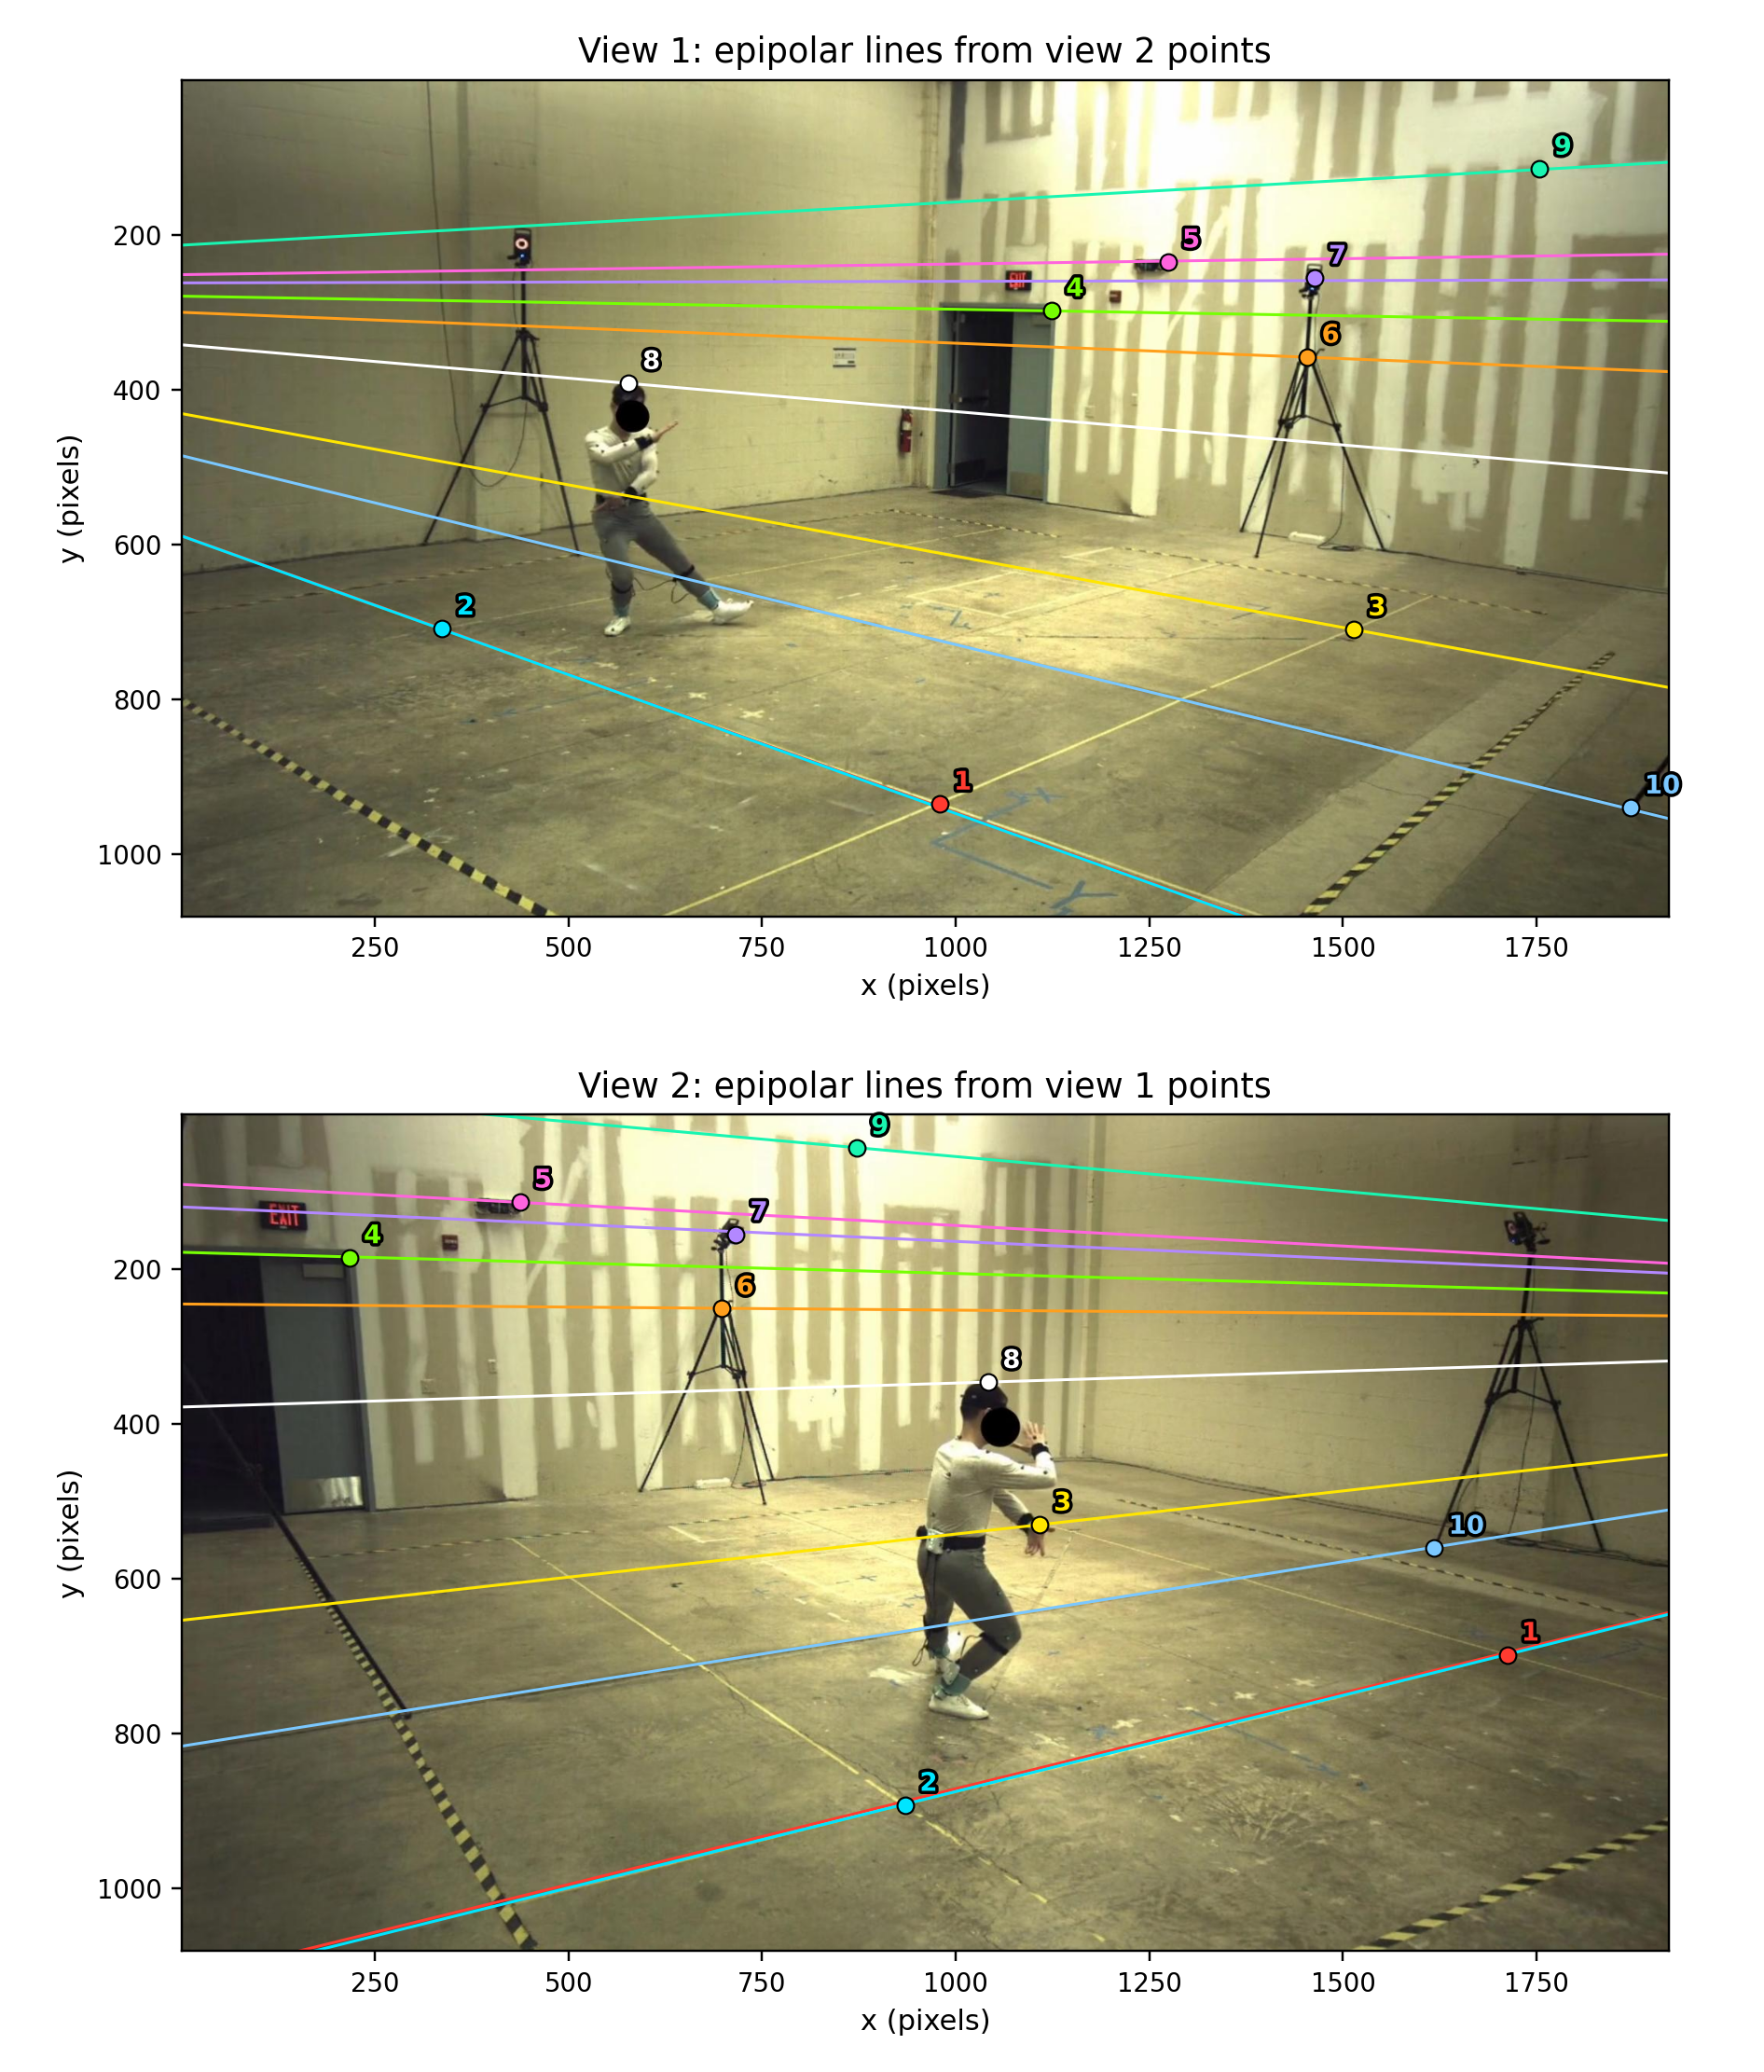
\includegraphics[width=0.86\textwidth]{figures/task3-5-report.png}
    \caption{Epipolar geometry from the known camera calibration. Top: image 1 points with lines $F^T \mathbf{p}_2$. Bottom: image 2 points with lines $F \mathbf{p}_1$.}
    \label{fig:task35-epipolar}
\end{figure}

\tasksection{Task 3.6}{Fundamental Matrix from Point Correspondences}
\label{sec:task3-6}

\subsection*{Method and slides reference}
We use the eight-point algorithm in \texttt{lecture18}: pages 8--12 construct the linear system, pages 13--19 derive its constrained least-squares solution, page 20 enforces rank two, and page 21 introduces coordinate normalization. The function \texttt{task3\_6} implements these steps using only the two sets of matched pixels; it does not use camera calibration.

The arrays in \texttt{main} contain ten manually selected point pairs, despite being named \texttt{eight\_pts1} and \texttt{eight\_pts2}. Two pairs were added to the initial eight after a large estimation error was observed. The reported result uses all ten pairs. The sampling images are in \texttt{eight\_points/}, with the additional pairs in \texttt{eight\_points/extra\_points/}. The points cover different parts and depths of the scene.

\subsection*{Coordinate normalization}
According to page 21 in the slide, the code subtracts each image's mean pixel coordinates and divides each coordinate by its standard deviation. For image $j$, let $\mu_{u,j},\mu_{v,j}$ be the means and $\sigma_{u,j},\sigma_{v,j}$ the standard deviations. Then
\[
    \widehat{\mathbf{p}}_j = T_j \mathbf{p}_j,
    \qquad
    T_j = \begin{bmatrix}
        1 / \sigma_{u,j} & 0 & -\mu_{u,j} / \sigma_{u,j}\\
        0 & 1 / \sigma_{v,j} & -\mu_{v,j} / \sigma_{v,j}\\
        0 & 0 & 1
    \end{bmatrix}.
\]
The call \texttt{std(pts,1,1)} uses division by the number of points when computing each variance. Both coordinate standard deviations are nonzero for the selected points.

\subsection*{Linear system and SVD solution}
For a normalized match $\widehat{\mathbf{p}}_1 = [u,v,1]^T$ and $\widehat{\mathbf{p}}_2 = [u',v',1]^T$, the row of $A$ is, as on page 11,
\[
    A_i = \begin{bmatrix}uu' & uv' & u & vu' & vv' & v & u' & v' & 1\end{bmatrix}.
\]
The unknowns are ordered by columns:
\[
    \mathbf{f} = (f_{11},f_{21},f_{31},f_{12},f_{22},f_{32},f_{13},f_{23},f_{33})^T.
\]
Thus $A_i \mathbf{f} = \widehat{\mathbf{p}}_2^T F_n \widehat{\mathbf{p}}_1$, and the ten matches form a $10\times9$ system. We use the lecture's solution of $\min_{\|\mathbf{f}\|_2 = 1}\| A \mathbf{f}\|_2^2$. Instead of explicitly forming $A^TA$, the code computes $A=U\Sigma V^T$. Since
\[
    A^T A = V \Sigma^T \Sigma V^T,
\]
the last column of $V$ is the eigenvector associated with the smallest eigenvalue.

\clearpage

\subsection*{Rank constraint and return to pixel coordinates}
As prescribed on page 20, the code takes the SVD of $F_n$, sets its smallest singular value to zero, and reconstructs the matrix. Denote this rank-two normalized matrix by $\overline F_n$.

To obtain the denormalization formula for our definitions of $T_1$ and $T_2$, substitute $\widehat{\mathbf{p}}_j = T_j \mathbf{p}_j$ into the normalized epipolar constraint:
\[
    \widehat{\mathbf{p}}_2^T \overline F_n\widehat{\mathbf{p}}_1 = (T_2\mathbf{p}_2)^T\overline F_n(T_1 \mathbf{p}_1) = \mathbf{p}_2^T \bigl(T_2^T \overline F_n T_1 \bigr)\mathbf{p}_1.
\]
Therefore the pixel-coordinate fundamental matrix is
\[
    F = T_2^T \overline F_n T_1.
\]
This gives the implementation \texttt{F = T2' * F * T1}. The left factor is the transpose of $T_2$, which maps pixels to normalized points. The code finally divides by \texttt{norm(F)}, the matrix 2-norm. This fixes the scale without changing the epipolar geometry.

\subsection*{Numerical result and visual verification}
The rounded result is
\[
    F = \begin{bmatrix}
        -5.617713523\times10^{-8} & 1.192218846\times10^{-6} & -0.000373151893\\
        1.517985352\times10^{-6} & 3.356509912\times10^{-7} & 0.001159820823\\
        -0.000218875280 & -0.004306292454 & 0.999989961720
    \end{bmatrix}.
\]
The function draws $\boldsymbol{\ell}_1 = F^T \mathbf{p}_2$ and $\boldsymbol{\ell}_2 = F \mathbf{p}_1$ using \texttt{draw\_epipolar\_lines}. Figure~\ref{fig:task36-epipolar} shows the ten input matches and their corresponding lines in both views. The points lie close to their lines and the pattern resembles the calibrated result in Task 3.5, so the geometry is reasonable. Small residual offsets remain because the points were selected by hand. Task 3.7 evaluates both matrices on the same 39 projected mocap matches, separately from these ten estimation pairs.

\begin{figure}[!htbp]
    \centering
    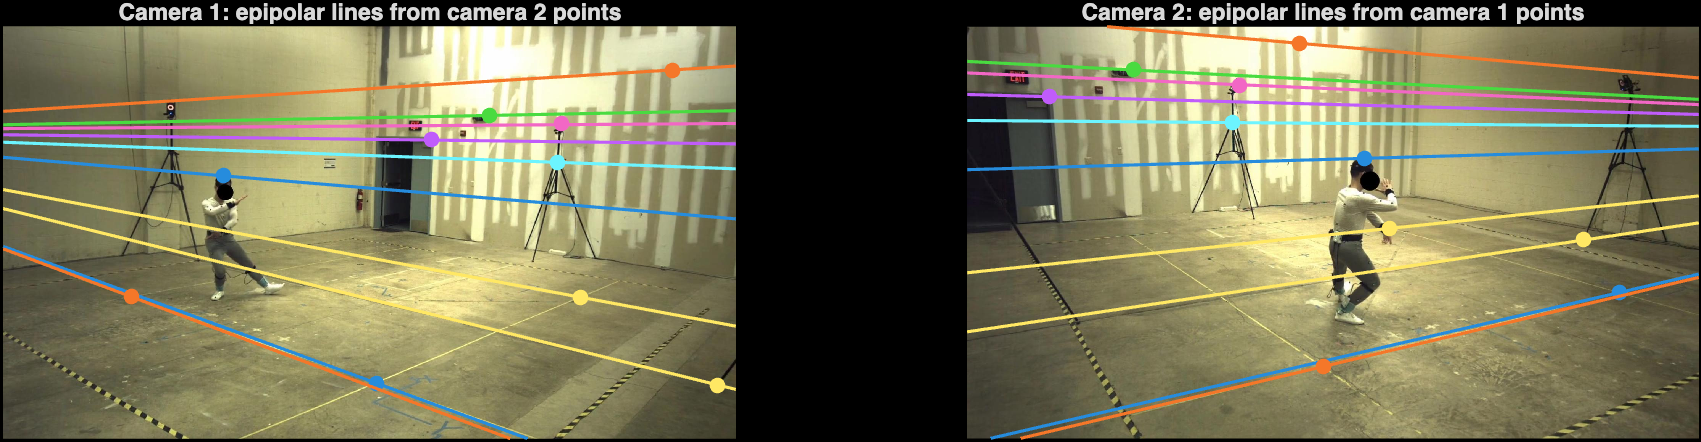
\includegraphics[width=\textwidth]{figures/task3-6-epipolar.png}
    \caption{Epipolar lines and ten manually selected matches from \texttt{task3\_6}. Left: camera 1 with $F^T \mathbf{p}_2$. Right: camera 2 with $F \mathbf{p}_1$.}
    \label{fig:task36-epipolar}
\end{figure}

\tasksection{Task 3.7}{Fundamental Matrix Evaluation}
\label{sec:task3-7}

\subsection*{Symmetric epipolar distance}
We evaluate both fundamental matrices on the same 39 accurate correspondences from Task 3.2. For each homogeneous pair $(\mathbf{p}_{1i},\mathbf{p}_{2i})$, \texttt{task3\_7} computes
\[
    \boldsymbol{\ell}_{1i} = F^T \mathbf{p}_{2i},
    \qquad
    \boldsymbol{\ell}_{2i} = F \mathbf{p}_{1i}.
\]
For a pixel $(u,v)$ and a line $\boldsymbol{\ell} = [a,b,c]^T$, the squared geometric distance is
\[
    d^2((u,v),\boldsymbol{\ell}) = \frac{(au+bv+c)^2}{a^2+b^2}.
\]
The function \texttt{calculate\_SED} computes these distances in each image and averages all $2n=78$ values:
\[
    \mathrm{SED}(F) = \frac{1}{2n} \sum_{i=1}^{n} \left[d^2(\mathbf{p}_{1i},\boldsymbol{\ell}_{1i}) + d^2 (\mathbf{p}_{2i},\boldsymbol{\ell}_{2i})\right].
\]
The computation uses the full-precision returned matrices, rather than the rounded entries displayed in this report.

\subsection*{Results and interpretation}
The recorded MATLAB run gives:
\begin{center}
\begin{tabular}{lc}
\toprule
Fundamental matrix & SED (pixels$^2$) \\
\midrule
Camera calibration, Task 3.5 & $1.73062429689\times10^{-26}$ \\
Ten-point estimate, Task 3.6 & $1.91669483902$ \\
\bottomrule
\end{tabular}
\end{center}

The calibration-based error is much smaller, as expected: the evaluation points were projected using the same camera parameters used to compute this $F$. The ten-point estimate is less accurate on these evaluation matches because it was obtained from manually selected pixels.

Taking the square root gives an RMS point-to-line distance of approximately $1.38$ pixels for the ten-point estimate. This suggests a search band of a few pixels as an initial scale for matching. The near-zero calibration result on synthetic projections does not imply that real and noisy image matches would have zero error.

\tasksection{Extra Task 1}{Camera Geometry for Cropped Views}
\label{sec:extra-1}

\subsection*{Objective and cropping rectangles}
We crop the two images to focus on the person while retaining all mocap points. The crop bounds below are given as $(x,y)$ pixel coordinates in the original images.

\begin{center}
\begin{tabular}{lccc}
\toprule
View & Top-left $(x_L,y_T)$ & Bottom-right $(x_R,y_B)$ & Width $\times$ height \\
\midrule
1 & $(515,374)$ & $(748,728)$ & $234\times355$ \\
2 & $(935,328)$ & $(1139,785)$ & $205\times458$ \\
\bottomrule
\end{tabular}
\end{center}

\subsection*{Transformation of pixel coordinates}
The top-left pixel of each crop becomes pixel $(1,1)$ in the cropped image. Thus, an original pixel $(x,y)$ inside the cropping rectangle has new coordinates
\[
    x' = x - x_L + 1, \qquad y' = y - y_T + 1.
\]
Using homogeneous pixel coordinates $\mathbf{p} = [x,y,1]^T$ and $\mathbf{p}' = [x',y',1]^T$, this translation can be written as
\[
    \mathbf{p}' = T\mathbf{p},
    \qquad
    T = \begin{bmatrix}
        1 & 0 & 1-x_L\\
        0 & 1 & 1-y_T\\
        0 & 0 & 1
    \end{bmatrix}.
\]
The translation depends on the crop origin, so the same $T$ applies to every point in that image. For the selected rectangles,
\[
    T_1 = \begin{bmatrix}
        1 & 0 & -514\\
        0 & 1 & -373\\
        0 & 0 & 1
    \end{bmatrix},
    \qquad
    T_2 = \begin{bmatrix}
        1 & 0 & -934\\
        0 & 1 & -327\\
        0 & 0 & 1
    \end{bmatrix}.
\]

\subsection*{Updated camera intrinsic matrices}
Let $\widetilde{\mathbf{X}} = [X,Y,Z,1]^T$ be a world point, and let $\texttt{Pmat}_j$ denote the extrinsic matrix of camera $j$. Its original projection satisfies
\[
    \lambda_j \mathbf{p}_j = K_j\, \texttt{Pmat}_j\, \widetilde{\mathbf{X}}.
\]
Multiplying by $T_j$ gives the projection into the cropped image:
\[
    \lambda_j \mathbf{p}'_j = (T_j K_j)\, \texttt{Pmat}_j\, \widetilde{\mathbf{X}},
    \qquad
    K_j' = T_j K_j.
\]
In particular, the intrinsic matrix becomes
\[
    K'_j = \begin{bmatrix}
        f_j a_j & s_j & c_{x,j} - x_{L,j} + 1\\
        0 & f_j & c_{y,j} - y_{T,j} + 1\\
        0 & 0 & 1
    \end{bmatrix}.
\]

\clearpage

\subsection*{Fundamental matrix for the cropped views}
We directly apply the result from Task 3.5. Cropping leaves the relative camera pose and essential matrix $E$ unchanged, so the fundamental matrix for the cropped views is
\[
    F' = (K'_2)^{-T} E (K'_1)^{-1}.
\]
For the selected crops, the result after the normalization used in \texttt{task3\_5} is approximately
\[
    F' = \begin{bmatrix}
        -9.947407735\times10^{-6} & 2.024800691\times10^{-4} & 0.007891075104\\
        2.392942257\times10^{-4} & 3.378792298\times10^{-5} & 0.343560976928\\
        0.037881712851 & -0.502220112294 & -0.811291647511
    \end{bmatrix}.
\]
\subsection*{Visual verification in the cropped images}
Figure~\ref{fig:extra1-crops} shows the projected points and the epipolar geometry in the cropped images. The top row uses all points. The bottom row displays six selected projected points and the epipolar lines.

\begin{figure}[!htbp]
    \centering
    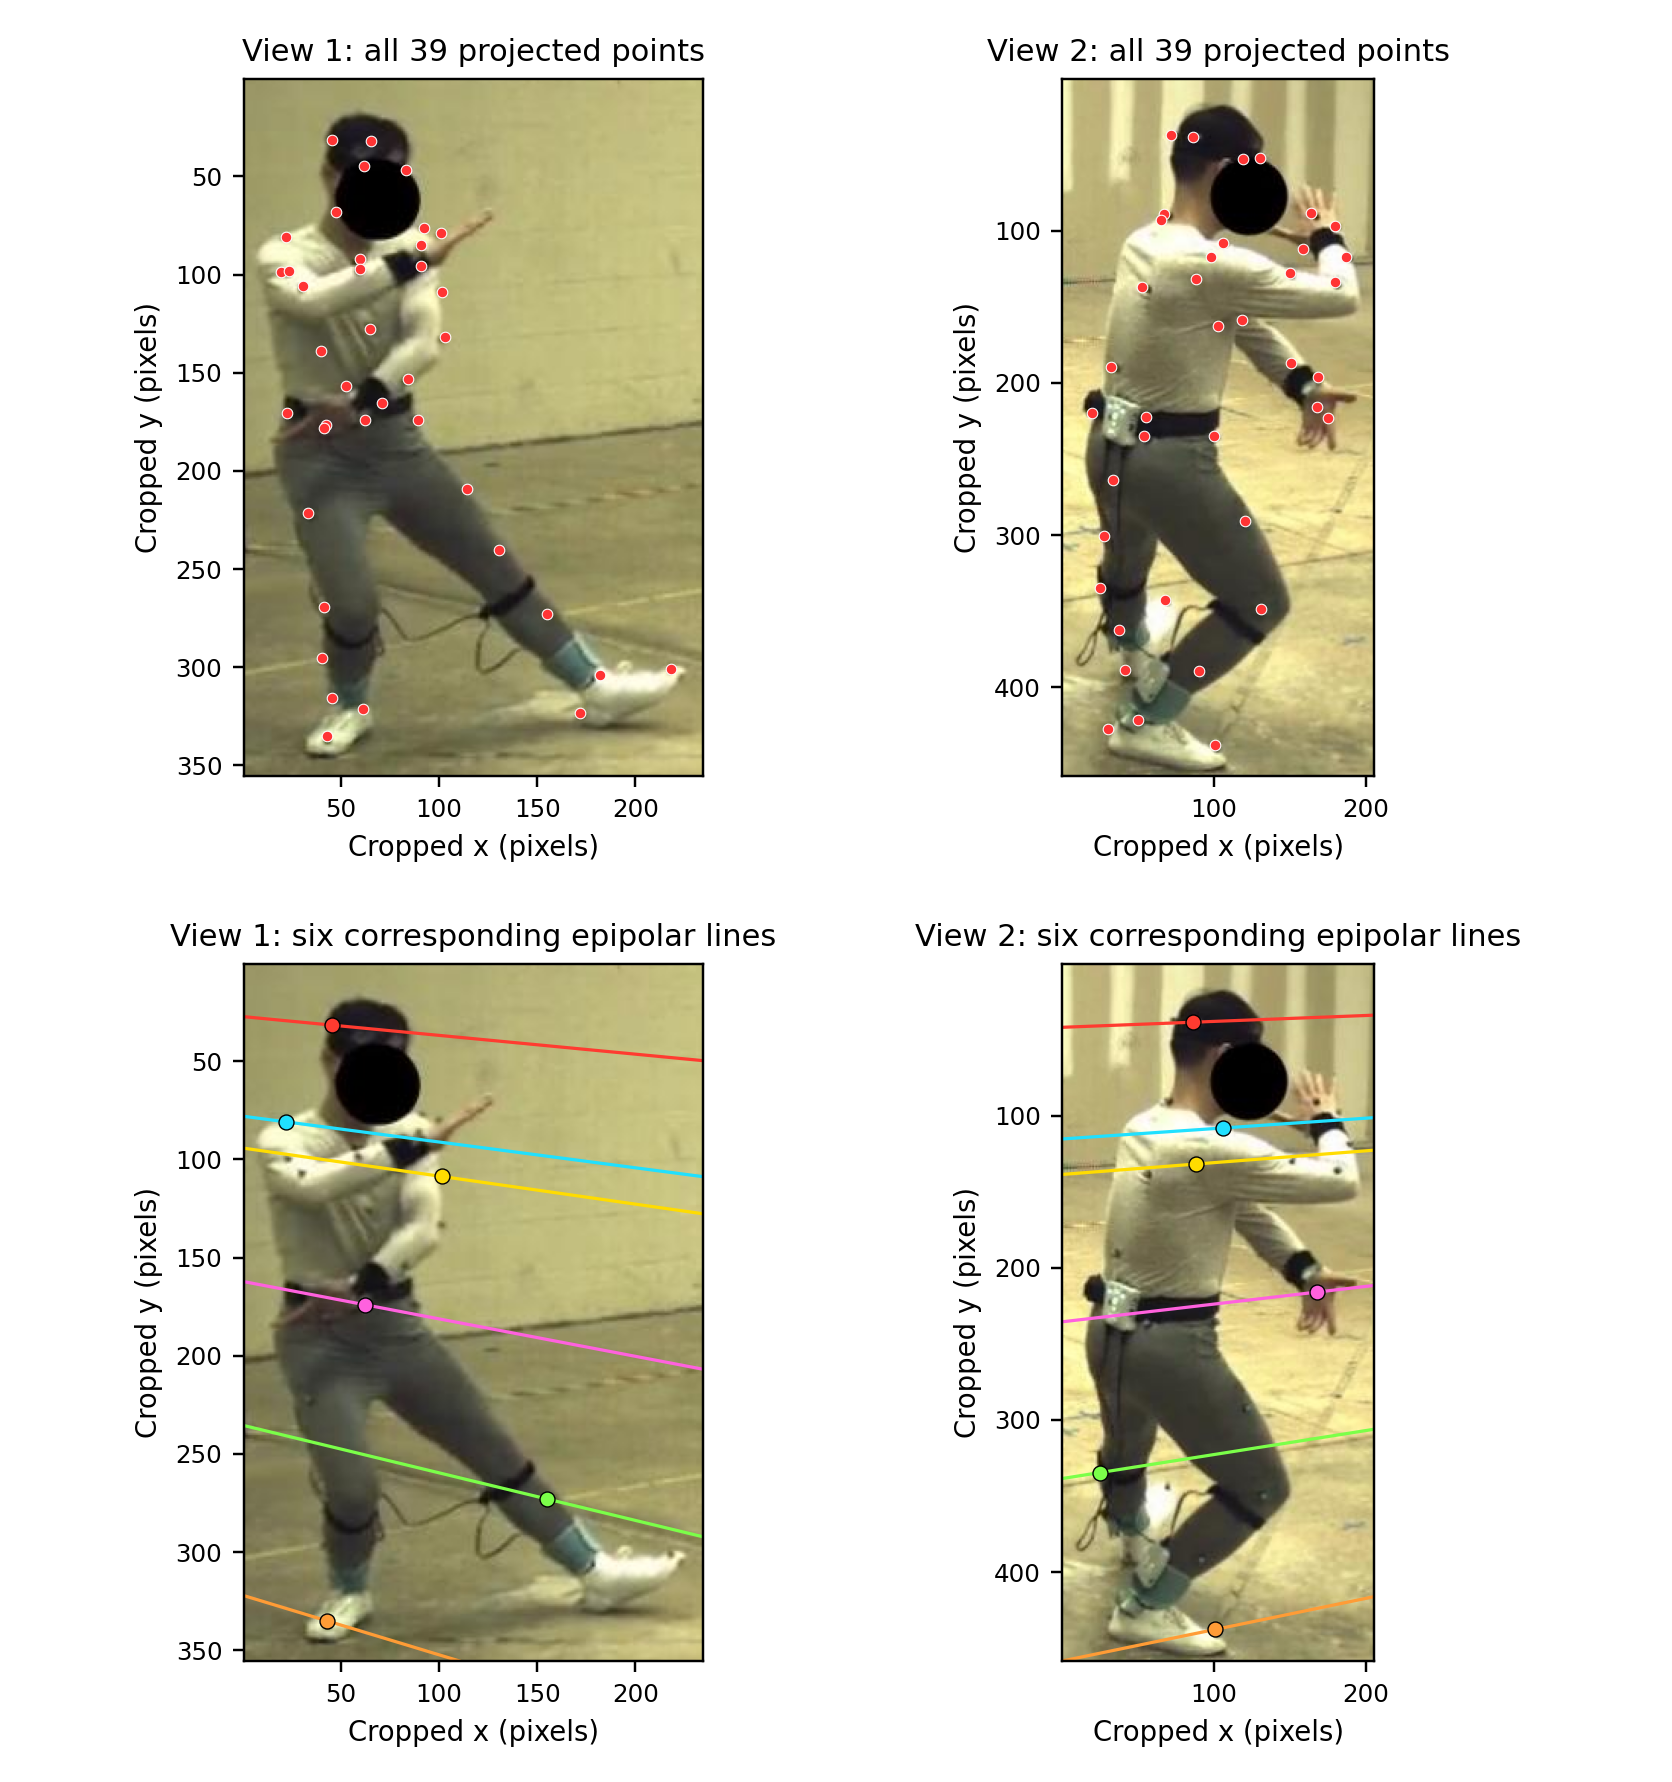
\includegraphics[width=0.73\textwidth]{figures/extra-1-report.png}
    \caption{Cropped views using the updated camera intrinsics and fundamental matrix. Top: all mocap points projected. Bottom: six selected projected points and the epipolar lines.}
    \label{fig:extra1-crops}
\end{figure}

\end{document}
